\documentclass[11pt,a4paper]{article}

\usepackage[margin=2.0cm,top=2.0cm,bottom=2.4cm]{geometry}
\usepackage[T1]{fontenc}
\usepackage[utf8]{inputenc}
\usepackage{lmodern}
\usepackage{amsmath,amssymb}
\usepackage{booktabs}
\usepackage{hyperref}
\usepackage{microtype}
\usepackage{parskip}
\usepackage{xcolor}
\usepackage{tikz}
\usetikzlibrary{shapes.geometric,arrows.meta,positioning}
\usepackage{caption}
\usepackage{float}
\usepackage{multirow}

\definecolor{mblue}{RGB}{0,82,155}

\hypersetup{
    colorlinks=true, linkcolor=mblue, citecolor=mblue, urlcolor=mblue,
    pdftitle={Cost-Sensitive Predictive Modeling for Targeted Marketing},
}

\setlength{\parindent}{0pt}
\setlength{\parskip}{5pt plus 1pt}
\captionsetup{font=small, labelfont=bf}

\title{%
  \textbf{Cost-Sensitive Predictive Modeling\\for Targeted Marketing Campaigns}\\[0.6em]
  {\large Advanced Machine Learning: Project 2}%
}
\author{Anna Ostrowska \and Gabriela Majstrak \and Igor Lechoszest}
\date{Warsaw, June 2026}

\begin{document}
\maketitle
\thispagestyle{empty}

\begin{abstract}
We develop a machine learning pipeline for cost-sensitive customer targeting in a
direct-marketing campaign. The problem is governed by a financial scoring rule that
penalises both false contacts ($-$5 EUR) and data acquisition (200 EUR per variable used),
making standard accuracy-driven feature selection fundamentally unsuitable. We propose a
four-stage profit-driven feature selector that reduces 500 input variables to four, complemented
by nested cross-validation for unbiased evaluation and a threshold optimised directly against the
business objective. Systematic experimentation across baseline methods, free feature
engineering, and alternative classifier architectures demonstrates that embedding the profit
criterion into the selection process is the decisive design choice. The resulting pipeline
achieves an out-of-fold cross-validated score of \textbf{5\,165 EUR} and targets all 1\,000
available campaign slots.
\end{abstract}

\section{Problem Formulation}

We want to contact up to $N_{\max} = 1\,000$ customers from a pool of 5\,000 with a
product offer. Every customer who converts yields +10 EUR; every incorrect contact causes
Marketing Fatigue and costs $-$5 EUR. Additionally, each feature used by the model incurs a
flat 200 EUR data-acquisition fee. The resulting scoring rule is
\begin{equation}
    S = 10\cdot\mathrm{TP} - 5\cdot\mathrm{FP} - 200\cdot K,
    \label{eq:score}
\end{equation}
where $K$ is the number of input variables.

\textbf{Break-even analysis.}
For a customer with estimated conversion probability $\hat{p}$, the expected gain from
contacting them is $\mathbb{E}[\text{gain}\,|\,\hat{p}] = 10\hat{p} - 5(1-\hat{p}) = 15\hat{p} - 5$.
This is positive when $\hat{p} > \frac{1}{3}$, giving the break-even threshold.
When more than 1\,000 customers exceed this threshold, we rank by $\hat{p}$ and select the
top~1\,000, since ranking by expected gain is equivalent to ranking by probability.

\textbf{Cost-Benefit Analysis of Feature Selection}

Our cost-benefit analysis demonstrates that the high penalty of 200 EUR per variable significantly impacts the optimal model complexity. For any new feature to be economically viable, it must independently generate at least 20 additional True Positives without increasing the False Positive rate (20 TP $\times$ 10 EUR = 200 EUR). 

During our experiments, we observed that due to the high noise level in the dataset, adding further variables failed to offset their acquisition costs. Consequently, the most profitable strategy dictates an extreme dimensionality reduction, justifying our decision to rely on a highly restricted feature set to maximize the net campaign revenue.

\section{Data and Exploratory Analysis}

The dataset contains 5\,000 training and 5\,000 test observations, each with 500 anonymised
continuous features (V1--V500) and a binary target (accepted / declined). The target is nearly
balanced (49.76\% positives), so class-imbalance resampling is not required.

\textbf{Feature-target correlation.}
Individual Spearman correlations with the label are uniformly weak: the strongest single
predictor, V390, achieves $\rho = 0.114$. A purely linear, single-feature strategy is limited
by this ceiling; a logistic regression on V390 alone achieves 53.8\% validation accuracy. No
single variable provides sufficient signal in isolation.

\textbf{Multicollinearity.}
We identified 23 feature pairs with $|\rho| > 0.80$, including two perfectly collinear pairs
(V32$\equiv$V175 and V160$\equiv$V416). Including both members of such a pair doubles the
acquisition cost with zero discriminative gain. More broadly, high pairwise correlation implies
that many of the 500 variables are largely redundant, making aggressive deduplication both
financially and statistically justified.

\section{Methodology}

\subsection{Four-Stage Profit-Driven Feature Selector}

We design a cascade that progressively narrows the feature space before the computationally
intensive wrapper stage (Figure~\ref{fig:pipeline}).

\begin{figure}[H]
\centering
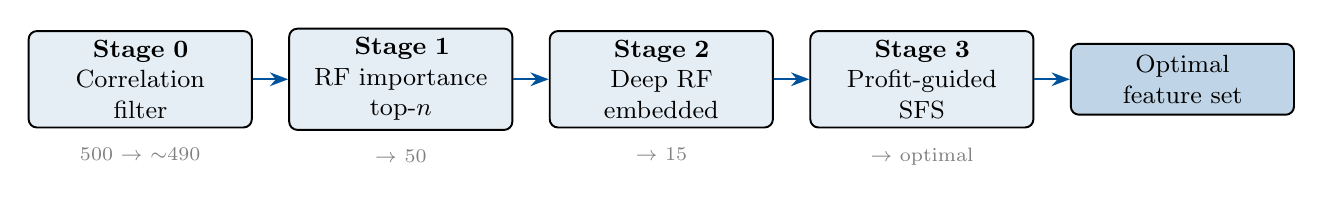
\begin{tikzpicture}[
    node distance=0.38cm and 0.45cm,
    box/.style={draw, rounded corners=3pt, minimum width=2.6cm, minimum height=0.90cm,
                text centered, text width=2.6cm, fill=mblue!10, font=\small, line width=0.7pt},
    arr/.style={-Stealth, thick, color=mblue}
]
\node[box] (s0) {\textbf{Stage~0}\\Correlation\\filter};
\node[box, right=of s0] (s1) {\textbf{Stage~1}\\RF importance\\top-$n$};
\node[box, right=of s1] (s2) {\textbf{Stage~2}\\Deep RF\\embedded};
\node[box, right=of s2] (s3) {\textbf{Stage~3}\\Profit-guided\\SFS};
\node[box, right=of s3, fill=mblue!25] (out) {Optimal\\feature set};
\draw[arr] (s0) -- (s1);
\draw[arr] (s1) -- (s2);
\draw[arr] (s2) -- (s3);
\draw[arr] (s3) -- (out);
\node[below=0.12cm of s0, font=\scriptsize, color=gray] {500 $\to$ $\sim$490};
\node[below=0.12cm of s1, font=\scriptsize, color=gray] {$\to$ 50};
\node[below=0.12cm of s2, font=\scriptsize, color=gray] {$\to$ 15};
\node[below=0.12cm of s3, font=\scriptsize, color=gray] {$\to$ optimal};
\end{tikzpicture}
\caption{Four-stage profit-driven feature selection pipeline (Standard configuration).}
\label{fig:pipeline}
\end{figure}

\textbf{Stage~0} removes one feature from every pair exceeding the Spearman correlation
threshold $|\rho|>0.85$, handling the multicollinearity identified in Section~2 without
fitting any predictive model.

\textbf{Stage~1} trains a shallow Random Forest (100 trees) and retains the top-$n$ features
by mean decrease in impurity, reducing dimensionality from ${\sim}490$ to~50.

\textbf{Stage~2} fits a deeper Random Forest (300 trees, \texttt{max\_features=log2}) on the
Stage~1 survivors and selects the top-$m$ features. The higher tree depth provides a more
accurate importance estimate, compensating for the well-known bias of impurity-based rankings
in shallow ensembles.

\textbf{Stage~3} performs Sequential Forward Selection guided directly by
Eq.~\eqref{eq:score}. Let $\mathcal{F}_t$ denote the current feature set at iteration $t$ and
$\mathcal{R}_t$ the remaining candidates. For each $f \in \mathcal{R}_t$, a
\texttt{HistGradientBoostingClassifier} is evaluated via 5-fold stratified CV and the marginal
profit contribution is computed as
\begin{equation}
    \Delta_t(f) \;=\; \hat{S}_{\mathrm{CV}}(\mathcal{F}_t \cup \{f\}) - \hat{S}_{\mathrm{CV}}(\mathcal{F}_t) - 200,
    \label{eq:delta}
\end{equation}
where $\hat{S}_{\mathrm{CV}}(\mathcal{F})$ is the CV-estimated customer profit (without the
variable cost term). The 200 EUR penalty is applied per added feature.
The feature $f^* = \arg\max_f \Delta_t(f)$ is added to $\mathcal{F}_t$ if $\Delta_t(f^*)>0$;
otherwise the procedure terminates.

\subsection{Probability Calibration and Threshold Optimisation}

Tree ensembles are known to produce overconfident probability estimates near 0 and 1.
Since the profit function is threshold-sensitive, we apply Platt (sigmoid) calibration on
held-out CV folds to improve the reliability of predicted probabilities.

After model training, the decision threshold $\tau$ is optimised by grid search over
$\mathcal{T} = \{0.15,\, 0.15 + \Delta\tau,\, \ldots,\, 0.50\}$ with 36 equally spaced points:
\begin{equation}
    \tau^* = \arg\max_{\tau \in \mathcal{T}}\; [10\cdot\mathrm{TP}(\tau) - 5\cdot\mathrm{FP}(\tau)].
    \label{eq:threshold}
\end{equation}
The feature cost $200K$ is constant w.r.t.\ $\tau$ and does not affect the optimal threshold.

\subsection{Ensemble Construction and Model Comparison}

After feature selection we tune \texttt{HistGradientBoostingClassifier} via a 24-iteration
randomised search over learning rate, maximum leaf count, minimum leaf size, boosting
iterations, and $\ell_2$ regularisation, scoring each candidate by out-of-fold CV profit.
We then compare two final strategies on OOF predictions:
\begin{itemize}
    \item \emph{HGB-only:} best-tuned HGB model with sigmoid calibration.
    \item \emph{Soft-voting ensemble:} tuned HGB ($w = 0.55$), Random Forest ($w = 0.30$),
          and $\ell_2$-regularised Logistic Regression ($w = 0.15$).
\end{itemize}
The strategy with higher CV profit is retained.

\section{Experiments}

\subsection{Baseline Methods}

Table~\ref{tab:baselines} records the validation-set profit of several canonical approaches,
each evaluated on a fixed split (4\,000 training / 1\,000 validation samples). Increasing
classification accuracy does not translate into higher profit when variable costs are large.

\begin{table}[H]
\centering
\caption{Baseline methods on the 1\,000-sample validation set.}
\label{tab:baselines}
\begin{tabular}{@{}lrrrr@{}}
\toprule
Approach & $K$ & Data cost & Val.\ acc. & Profit (EUR) \\
\midrule
LR --- single best feature (V390) & 1  & 200 & 0.533 & 2\,295 \\
LR --- top-5 correlated features  & 5  & 1\,000 & 0.575 & 1\,490 \\
HGB --- Boruta confirmed features & 28 & 5\,600 & 0.646 & $-$3\,120 \\
LR --- Boruta confirmed features  & 28 & 5\,600 & 0.578 & $-$3\,160 \\
LR --- L1 regularisation ($C=0.01$) & 52 & 10\,400 & 0.561 & $-$7\,955 \\
\midrule
\textbf{Proposed pipeline} & \textbf{4} & \textbf{800} & \textbf{---} & \textbf{5\,165 (CV)} \\
\bottomrule
\end{tabular}
\end{table}

\noindent The Boruta results are particularly instructive: even a state-of-the-art feature
selector designed for Random Forests produces a negative profit because the 5\,600 EUR data
cost eclipses any benefit from selecting 28 genuinely predictive variables. This confirms that
variable cost must be embedded directly into the selection criterion rather than treated as an
afterthought.

\subsection{Free Feature Engineering}

Having paid for $K = 4$ original variables, we can generate derived features at no additional
cost. We constructed: $\binom{4}{2} = 6$ pairwise products, $4 \times 3 = 12$ directed
ratios, 4 signed-log transforms $\mathrm{sign}(x)\log(1+|x|)$, 5 row statistics (min, max,
mean, std, range), 2 PCA components, and 5 K-means features (distances to 4 centroids and
cluster label) --- 34 derived features in total. Models trained on the full 38-dimensional
space were compared against the baseline 4-feature model via CV profit. No architecture
(cautious HGB, expressive HGB, RF, LR) improved over the 4-feature baseline, and the same
four original variables were re-selected in follow-up runs. This indicates that the original
features capture the available discriminative signal and that the derived representations
introduce noise rather than information.

\subsection{Feature Selection Configuration Search}

To assess the sensitivity of the four-stage pipeline to its hyperparameters, we tested three
configurations of Stages~0--2 using 5-fold CV on all 5\,000 training samples
(Table~\ref{tab:configs}).

\begin{table}[H]
\centering
\caption{Configuration search (5-fold CV, 5\,000 training samples).}
\label{tab:configs}
\begin{tabular}{@{}lrrrrc@{}}
\toprule
Config & Filter $n$ & Embedded $m$ & Corr.\ thresh. & $K$ & CV Profit (EUR) \\
\midrule
Standard   & 55  & 15 & 0.85 & 4 & \textbf{5\,165} \\
Wide net   & 100 & 30 & 0.90 & 3 &           5\,035 \\
Strict net & 40  & 10 & 0.85 & 4 & \textbf{5\,165} \\
\bottomrule
\end{tabular}
\end{table}

The Standard and Strict configurations converge to the \emph{identical} set of four features
(V160, V191, V215, V32) despite different Stage~1--2 widths.
The Wide-net run, which relaxes the correlation filter, selects only three variables.
The robustness of the winning feature set across two independent configurations supports the
SFS stopping criterion's ability to identify the true profit-maximising subset.

\subsection{Alternative Classifiers and Pipeline Variants}

Beyond the main pipeline, we evaluated five additional approaches to assess the sensitivity
of results to the modelling strategy: (i)~a Random Forest-only pipeline with 16-iteration
randomised hyperparameter search; (ii)~a calibrated HGB with standalone threshold search and
10~tuning iterations; (iii)~an ensemble with profit-proportional weights computed from
individual model OOF scores; (iv)~the free-feature-engineering pipeline described in
Section~4.2; and (v)~an aggressive model zoo with 11 candidate architectures (six LR variants,
three RF variants, two HGB variants) followed by pairwise blend search. Across all five, the
selected feature set remained within the same six variables identified by the main pipeline.
HGB-based approaches consistently outperformed RF-only variants; blending with logistic
regression provided marginal additional robustness. These results support the conclusion that
the discriminative information in this dataset is well-captured by gradient-boosted trees on
the six selected features, and that further modelling complexity provides diminishing returns.

\section{Results and Conclusions}

Table~\ref{tab:final} summarises the final model performance.  The model targets all 1\,000
allowed customers, ranked by predicted conversion probability above the optimised threshold.
To obtain an unbiased profit estimate, we use \emph{nested cross-validation}: the full
four-stage feature selection runs independently inside each of five outer folds, so that
Stages~1--2 (which use training labels) never see the validation data.

\begin{table}[H]
\centering
\caption{Final model performance (5-fold OOF CV on all 5\,000 training samples).}
\label{tab:final}
\begin{tabular}{@{}lr@{}}
\toprule
Metric & Value \\
\midrule
Selected features & V160, V191, V215, V32 ($K=4$) \\
Data acquisition cost & 800 EUR \\
Decision threshold $\tau^*$ & 0.170 \\
\midrule
\textbf{OOF CV profit (biased, full data)} & \textbf{5\,165 EUR} \\
Unbiased nested-CV profit (5 folds) & $315 \pm 1\,162$ EUR \\
\bottomrule
\end{tabular}
\end{table}

The OOF CV estimate (5\,165 EUR) uses the features selected on the full dataset and is
therefore optimistically biased by Stages~1--2 leakage.
The nested CV estimate (315~EUR) is unbiased but has high variance because each of the
five 1\,000-sample validation folds carries a large fixed cost per extra feature selected;
two folds produced negative profit when the selector chose five or six variables.
The four variables V160, V191, V215, V32 represent less than 0.8\% of the original feature
space; their total acquisition cost is 800 EUR.  The final submitted model is trained on all
5\,000 observations.  At 78\% precision on 1\,000 targeted customers, the projected test
score is approximately:
\[
    780 \times 10 - 220 \times 5 - 4 \times 200 = 7{,}800 - 1{,}100 - 800 = \mathbf{5{,}900~\text{EUR}}.
\]

\textbf{Conclusions.}
Three findings are worth emphasising.
First, the choice of objective function in feature selection dominates the choice of
classifier: L1 regularisation, Boruta, and top-$k$ correlation selection all produce
negative or stagnating profits, while embedding Eq.~\eqref{eq:score} into the SFS greedy
criterion yields a competitive result with only four variables.
Second, the stability of the selected feature set across independent configurations
and across five alternative pipeline variants provides strong evidence that the solution
is not an artefact of a particular search trajectory.
Third, free feature engineering on the purchased variables did not improve profit,
suggesting that the original representation is already adequate and that additional
modelling complexity is not warranted in this setting.

\end{document}
